% to choose your degree
% please un-comment just one of the following
\documentclass[bsc,frontabs,twoside,singlespacing,parskip,deptreport]{infthesis}     % for BSc, BEng etc.
% \documentclass[minf,frontabs,twoside,singlespacing,parskip,deptreport]{infthesis}  % for MInf

\usepackage{hyperref}
\usepackage{cite}
\usepackage{amsmath}
\usepackage{graphicx}
\usepackage{caption}
\usepackage{subcaption}
\usepackage{wrapfig}

\begin{document}

\title{Targeted Influence in Social Networks}

\author{Lewis Barker}

% to choose your course
% please un-comment just one of the following
%\course{Artificial Intelligence and Computer Science}
%\course{Artificial Intelligence and Software Engineering}
%\course{Artificial Intelligence and Mathematics}
%\course{Artificial Intelligence and Psychology }   
%\course{Artificial Intelligence with Psychology }   
%\course{Linguistics and Artificial Intelligence}    
\course{Computer Science}
%\course{Software Engineering}
%\course{Computer Science and Electronics}    
%\course{Electronics and Software Engineering}    
%\course{Computer Science and Management Science}    
%\course{Computer Science and Mathematics}
%\course{Computer Science and Physics}  
%\course{Computer Science and Statistics}    

% to choose your report type
% please un-comment just one of the following
%\project{Undergraduate Dissertation} % CS&E, E&SE, AI&L
%\project{Undergraduate Thesis} % AI%Psy
\project{4th Year Project Interim Report}

\date{\today}

\abstract{
Abstract goes here.
}

\maketitle

\section*{Acknowledgements}
Acknowledgements go here. 

\tableofcontents

%\pagenumbering{arabic}


\chapter{Introduction}


\chapter{Background}
\section{Related Works}
ToDo

\chapter{Work Done}
\section{Formal Definitions}

\subsection{Input}
Initially we are given a \textbf{graph} $G = (V, E \subseteq V \times V)$ and $k$ \textbf{messages} $ m_{1} ... m_{k}$, which have \textbf{sources} $s_{1} ... s_{k}$ and \textbf{destinations} $d_{1} ... d_{k}$. 

The graph $G$ represents the social network, with vertices in $V$ being the users of the network and edges in $E$ being connections between users within the network. A connection between two users $a$ and $b$ means in our context that user $a$ may see some content shared by user $b$ - however whether they actually see it or not is decided by the social network's algorithm.

\subsection{Rounds}
The system progresses in a series of \textbf{rounds}, representing periods of time passing in which messages can be passed on to other users. This allows us to more easily reason about the flow of information and also simulate the process.

For any round $t$, and for some vertex $v \in V$, the \textbf{shared set} $S_{t}(v)$ is the set of messages which were shared by $v$ in that round.

We assume that the source of a message will invariably share it initially (otherwise it has no chance to propagate). Therefore initially, at round 0, for each $v \in V$ the shared set is defined as the set of messages for which $v$ is the source:

\begin{equation}
S_{0}(v) = \{m_{x} \; | \; x \in [0, k] \wedge s_{x} = v\}
\end{equation}


We also define, for each $v \in V$ at any round $t > 0$, the \textbf{possible set} as all of the messages shared by neighbours of $v$ in the previous round - all the messages which $v$ may be able to see at this point:

\begin{equation}
P_{t}(v) = \bigcup_{u \in N(v)} \quad \bigcup_{m \in S_{t-1}(u)} (u, m)
\end{equation}

In the above equation, $N(v)$ is the set of neighbouring vertices of v, and $(u, m)$ is a 2-tuple. Given a tuple $p = (u, m)$, we say that $p_{(1)} = u$ and $p_{(2)} = m$, as a way of accessing the parts of the tuple.

Which of these messages are actually shown to $v$ is determined by the social network's algorithm - which is what we wish to design. We define the \textbf{shown set} of a user $v$ at some round $t$, $T_{t}(v)$, as the result of this algorithm - this will be a subset of the possible set for that user and round:

\begin{equation}
T_{t}(v) \subseteq P_{t}(v)
\end{equation}

Finally, from the messages that are shown to a user, the user will share some of them. This is decided by the user model algorithm. The result of this form the \textbf{shared set} of that user for this round - all messages in the user's shared set must have been part of their shown set for that round:

\begin{equation}
\forall m \in S_{t}(v) . \exists (u, n) \in T_{t}(v) . m = n
\end{equation}

This is then used as the basis for the possible set of neighbouring vertices in the next round. With this, we need only define the showing and user model algorithms to be able to simulate the spread of messages throughout the network.

\section{Simulation Program}
For the purpose of running simulations of message spread in networks, a program was written allowing for running various simulations and receiving relevant results. The program was written in Python, using the NetworkX library [reference?] to represent and manipulate the network graphs. The program is split into classes, many of which have abstract base classes, to allow for easily creating different versions to swap in and out.

There is a \texttt{GraphGenerator} abstract base class, subclasses of which encapsulate the knowledge specific to the graph model being used - including how to create a graph of that type, and how the nodes should be positioned in the visualisation (for example if the network is based on a grid layout, it should be positioned as such). The rest of the program is totally independent from this knowledge, meaning that by simply using a different subclass the graph generation method can be modified completed - for example the graph could be loaded from a static file.

The showing algorithms are contained within subclasses of the \texttt{ShowModel} class, the main method of which is \texttt{show\_alg} which given a user's possible set and some additional information about the state of the network, returns a subset of the messages to be shown to them. Similarly, the user models algorithms are represented by subclasses of the \texttt{ShareModel} class, which has a method \texttt{share\_alg} to take the shown set and return the messages which the user will share. Changing which of these subclasses is used in the simulation allows comparing the performance of different algorithms.

These classes are brought together by the \texttt{Simulation} class, which is given an instance of each of \texttt{GraphGenerator}, \texttt{ShowModel}, and \texttt{ShareModel} on creation. The simulation can then be either run once or repeated multiple times, collating the results. When repeating the simulation, it can set to either use the exact same network graph or to regenerate the graph using the same generation method - in the case of randomly generated graphs, this allows for repeating the simulation to remove random differences caused by specific graphs. The simulation class can also create visualisations as outputs. It can output either images of the state at each round of the simulation, or a single video of the entire simulation. In these visualisations, a single message is highlighted as it spreads through the network, while the other vertices are coloured based on their level of traffic. This allows for seeing how a message moves through the graph and how far it spreads, as well as where potential bottlenecks occur and how busy the network is as a whole.

\section{Network Graph}
An important factor in how a message showing algorithm performs is the network that it is being performed on. If the network has invalid properties, the a successful algorithm may not be successful on other networks.

For the majority of this project, Kleinberg's model for small world graphs was used\cite{Kleinberg00}. This is a model which randomly creates a graph that fits certain properties. Initially, nodes are arranged in a grid layout, with a "grid distance" from each other. Each node is connected to its immediate neighbours (those a grid distance of 1 away). Each node is then connected to a constant number $k$ of other nodes. The probability of connecting node $u$ to node $v$ in this way is proportional to $d(u, v)^{-q}$ where $d(u, v)$ is the grid distance between $u$ and $v$, and $q$ is a constant affecting how likely the links are to be "far-reaching". If $q$ is 0, then the node will be linked to other nodes uniformly. If $q$ is high, the long links are more likely to connect closer nodes.

\begin{figure}[ht]
  \centering
    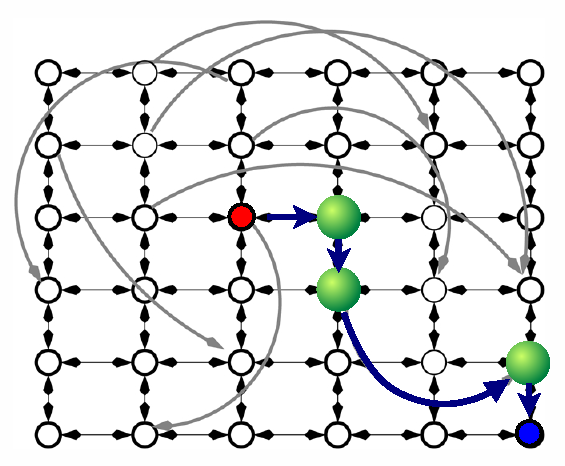
\includegraphics[width=0.5\textwidth]{Schabanel11_Kleinbergs_Network}
  \caption{A Kleinberg Graph with an example of the distributed greedy search\cite{Schabanel11}}
\end{figure}

This model provides several properties which make it suitable to use in place of a social network. Since it is randomly generated, we can run experiments using multiple different graphs to avoid results being skewed by peculiarities of individual networks. 

Additionally it fits into a category of graphs know as "Small World" graphs. This is related to Milgram's famous "Six Degrees of Separation" experiment\cite{Milgram67,TraversMilgram69}, in which he randomly chose individuals and asked them to forward a message on to a certain "target" via people they knew. Of those messages that reached the target, the median number of "steps" required was 6, displaying the existence of short paths within social networks - a fact that has also been seen in other studies\cite{MilgramBackup1,MilgramBackup2}. In addition to these paths existing, the experiment showed that it was possible for the intermediate individuals to find these paths without knowing the full structure of the network - they were able to conduct a distributed search. 

Kleinberg's model replicates both of these properties. For $q = 2$ and $k \ge 1$ the expected diameter of a graph generated using this model is $\theta (\log n)$ and a route between two nodes can be found in a distributed manner using $\theta (\log^{2}n)$ steps\cite{AnalyzingKleinberg}. This is achieved by sending the message as close as possible to the destination (in terms of grid distance) at each step.

This can be related to real networks intuitively. Individuals are more likely to be connected to those "close" to them - which in turn forms clusters of connections - but there will also be some "long-distance" connections that can connect clusters. To send a message to a far away target, a reasonable strategy would be to send to the person you know who is "closest" to the target - they are more likely to be connected to them.

While Kleinberg's small world model has been used primarily up to this point, other graph types may provide additional interesting insights. For example, using a plain grid could provide a baseline for what can be expected, to see if the algorithm developed takes advantage of the long link properties of the network. Alternatively, an real social network dataset could be used to see if the algorithm also work in actual networks.

\section{User Models}
While the main focus of this project was on the effect of the social network's "showing" algorithm, the model used also requires an algorithm to represent the user's actions. This algorithm should decide which of the messages shown to a user they then share - it chooses $S_{t}(v)$ based on $T_{t}(v)$. Depending on how this decision is modelled, it can add an element of uncertainty or randomness to the system, affecting which "showing" algorithms perform well.

\subsection{Basic User Model}
Initially, a very basic random selection method was used to choose the $S_{t}(v)$. Firstly, the user only considers the top $a$ of the messages shown to them (or all of the messages if there is less than $a$), where $a$ is a global constant - this represents the user's "attention", being unable to look at every message shown to them [expand on this?][reference attention paper?]. In the implementations used, the value of $a$ is also known to the showing algorithm, which does not show more than this many messages. From these $a$ messages, $b$ are selected at random and shared (or all of them are shared if there are less than $b$), where $b$ is a global constant and $b \le a$.

This provides us with a degree of randomness - if there are more than $b$ messages shown to the user, we can't tell which ones will be passed on. However in the case where there are less than or equal to $b$ messages shown to the user, this model acts unrealistically - the user will share every message they see. A real social network user would likely be less predictable (unless there was some incentive to share messages), and may not share all of the messages in nay circumstances. As a result of this unnatural behaviour, showing each message to only a single user at each step was found to be a highly effective strategy - however in a real situation this would likely result in losing the message at an uncooperative user.

\subsection{Probabilistic User Model}
A more realistic user model can be created using more probabilistic methods. In this user model, the concept of a maximum attention of $a$ is retained, with the user considering up to $a$ messages. However from these $a$ messages, rather than choose a set amount at random each message is shared with a probability $p$, where $p$ is a global constant.

This results in a situation where a user may share all the messages they see, or may share none. This emulates how a user will only share certain messages based on some criteria unknown to the network. With this model, if messages are not sent to enough users then they are likely to not be shared and be lost.

\section{Showing Models}
The key part of this project is the algorithm which decides which messages to show to each user. Users have "attention" limits, meaning that they will only look at a certain (globally constant) number of messages each round. This means that we can't just pass on every message - we need to prioritise. Each user is therefore only shown messages up to the "attention limit" to represent this. By changing which messages are shown we can attempt to direct messages to their recipients, preferably without clogging up the network with numerous duplicates and without losing the message by not duplicating it enough.

So far, several simple algorithms have been investigated, using basic heuristics to decide whether or not to show a message to a user.

\subsection{Algorithm 1: Any Closer Node}
In the first algorithm used, for each node we first select candidate messages that might be shown to them. A message is made a candidate if it has not already been delivered, and the receiving node (the one potentially being shown the message) is closer to the message's final target than the previous node was (the one that shared the message in the previous round, causing this message to be part of the possible set). After candidates have been selected, if there are more messages than can be shown to the node, the maximum amount are chosen randomly from the candidates. More formally:

\begin{equation}
\begin{split}
candidates = \{ (u, m_{k}) \in P_{t}(v) \:\: | \:\: & D(v, d_{k}) < D(u, d_{k}) \: \wedge \\
& m_{k} \mbox{ has not been delivered} \}
\end{split}
\end{equation}

\begin{equation}
T_{t}(v) = sample(candidates, max(|candidates|, a))
\end{equation}

Where $D(u, v)$ is the grid (Manhattan) distance between $u$ and $v$, $sample(x, n)$ randomly samples $n$ values from the collection $x$, and $a$ is the maximum messages that can be shown to any node (their attention span).

Note that if a message is in the possible set multiple times (from different previous nodes), it may be shown to the user multiple times (once for each previous node). Depending on the user model, this may increase the probability of it being shared by them.

\subsection{Algorithm 2: Further Nodes With Probability}
The second algorithm is a modification of the first with the intention of allowing the messages to spread in other directions not necessarily towards their destination. This may help prevent the message from dying out if the "direct" route is very busy.

In this algorithm, we again select candidates to be shown to each node. Again, messages are only made candidates if they have not been delivered. Of those undelivered messages, any for which the receiving node is closer to the destination than the previous node are made candidates, as before. Additionally, messages which will not get closer to their destination are made candidates with a globally constant probability $p$. As before, if there are too many candidates then the correct amount are chosen at random. More formally:

\begin{equation}
\begin{split}
candidates = \{ (u, m_{k}) \in P_{t}(v) \:\: | \:\: & (D(v, d_{k}) < D(u, d_{k}) \: \vee \: r < p) \: \wedge \\
& m_{k} \mbox{ has not been delivered} \}
\end{split}
\end{equation}

\begin{equation}
T_{t}(v) = sample(candidates, max(|candidates|, a))
\end{equation}

Where $0 \leq p < 1$ is a globally constant probability and $0 \leq r < 1$ is a randomly chosen value.

Note that if $p$ were to be set to 0, Algorithm 2 would behave the exact same as Algorithm 1.

\subsection{Algorithm 3: Only Single Best Node}
The third algorithm tested uses a simpler concept - each message is passed on to at most one other node, the node which is determined to be the "best" next step. This provides a basis for comparison with the case where messages are never duplicated.

Candidate messages are again selected for each node. In this algorithm a message is a candidate if it has not yet been delivered, and if that node is the "best" next step for the message. We define the "best" next step as the neighbour of the previous step which is closest to the target in grid distance, and in the case of a draw has the lowest node index (to ensure that the "best" next step is consistent). If there are too many candidates then the first up to the limit are taken. Since we are not worried about spreading messages "fairly" as they do not duplicate, this doesn't need to be chosen randomly. Formally:

\begin{equation}
\begin{split}
candidates = \{ (u, m_{k}) \in P_{t}(v) \:\: | \:\: & isBest(m_{k}, u) \: \wedge \\
& m_{k} \mbox{ has not been delivered} \}
\end{split}
\end{equation}

\begin{equation}
T_{t}(v) = candidates[:a]
\end{equation}

Where $isBest(m, u)$ is a predicate which is true if node $u$ is the best next step for message $m$, and $x[:a]$ is the first $a$ items in $x$.


\chapter{Results}
After development of the algorithms, experiments were run to compare their performance. All simulations were run on a 20 by 20 graph generated using Kleinberg's model, with parameters $k = 1$ and $q = 2$. They were simulated for 25 rounds, which was found in all cases to be enough time for any activity to stop. 

\begin{wrapfigure}{L}{0.65\textwidth}
  	\vspace{-25pt}
    \centering
    \begin{subfigure}[b]{0.3\textwidth}
        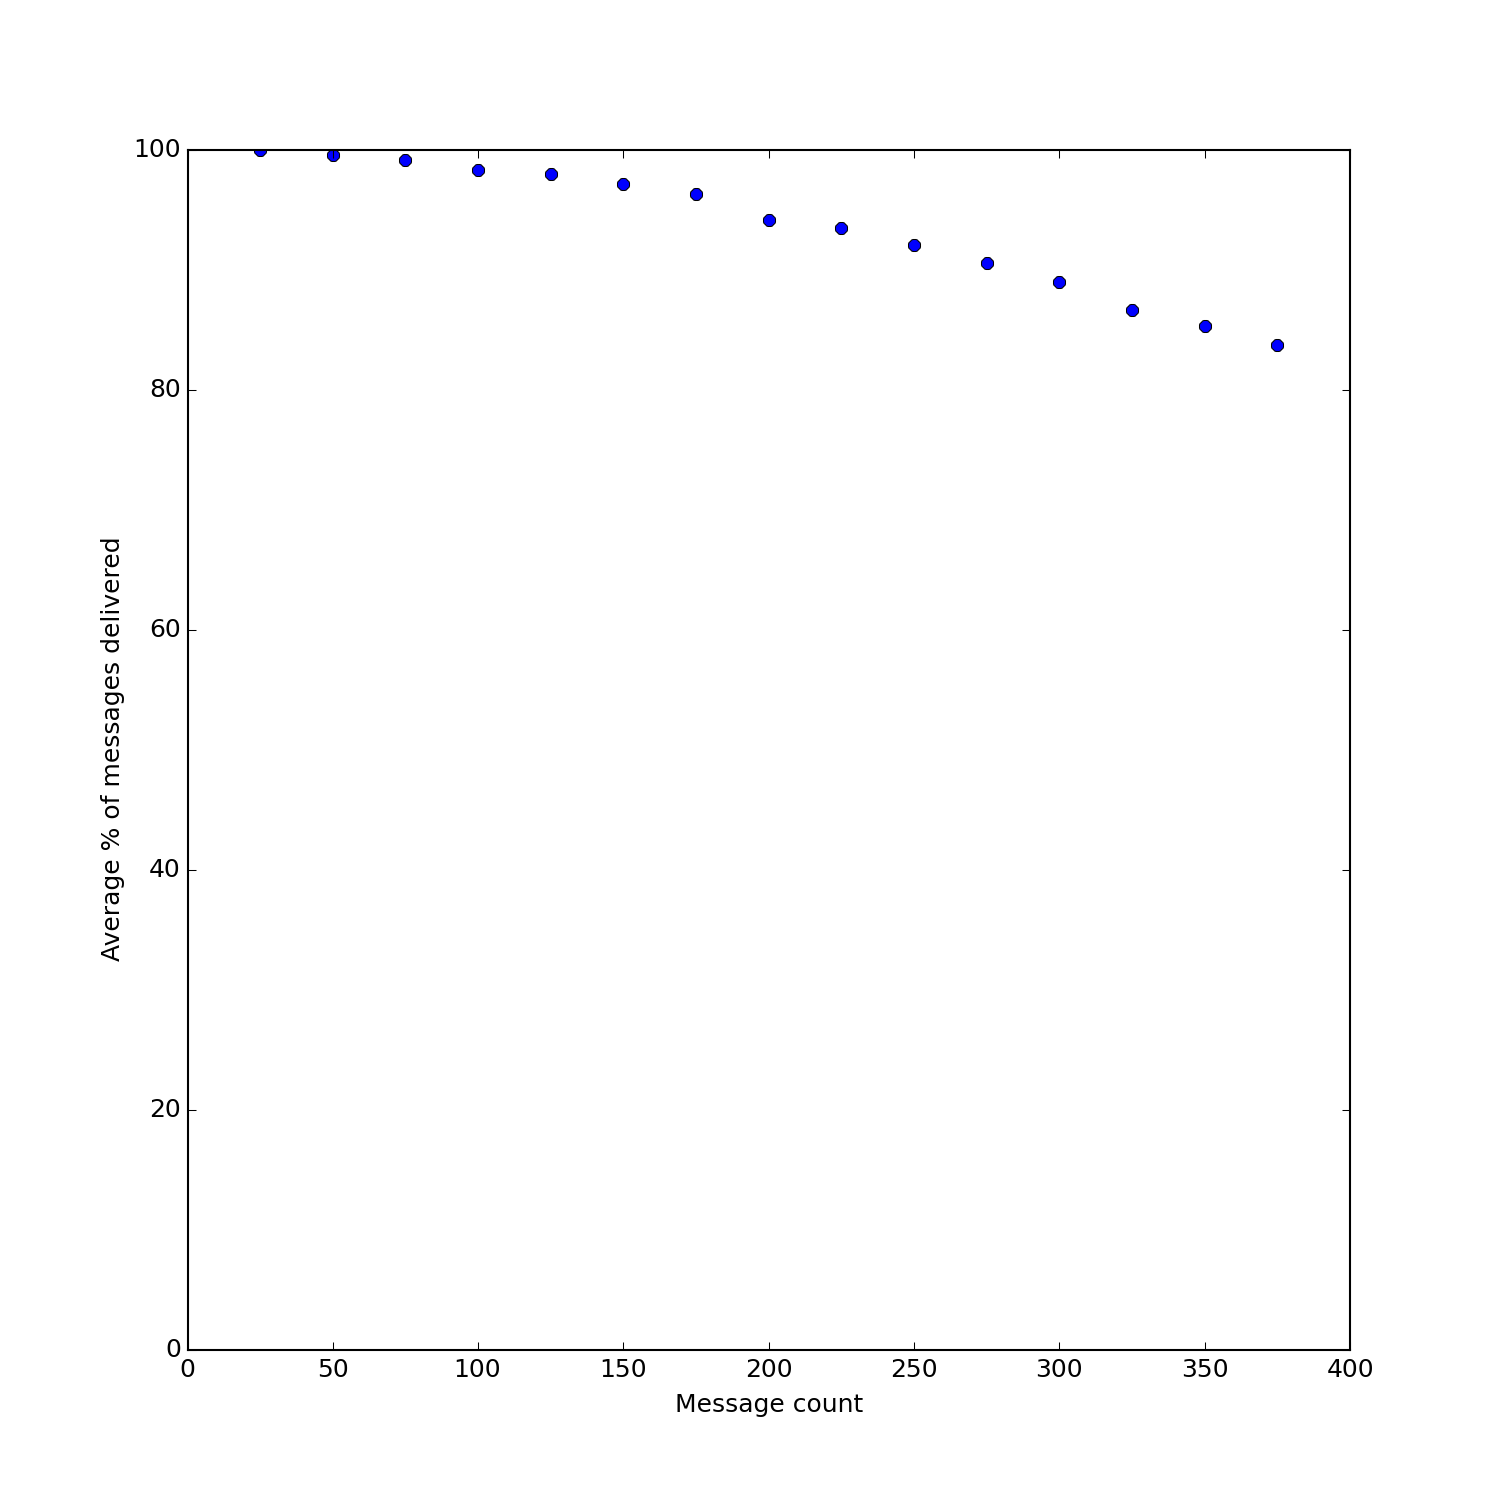
\includegraphics[width=\textwidth]{results/BasicShare_Prob0}
        \caption{Algorithm 1}
        \label{fig:results/BasicShare_Prob0}
    \end{subfigure}
    ~ %add desired spacing between images, e. g. ~, \quad, \qquad, \hfill etc. 
      %(or a blank line to force the subfigure onto a new line)
    \begin{subfigure}[b]{0.3\textwidth}
        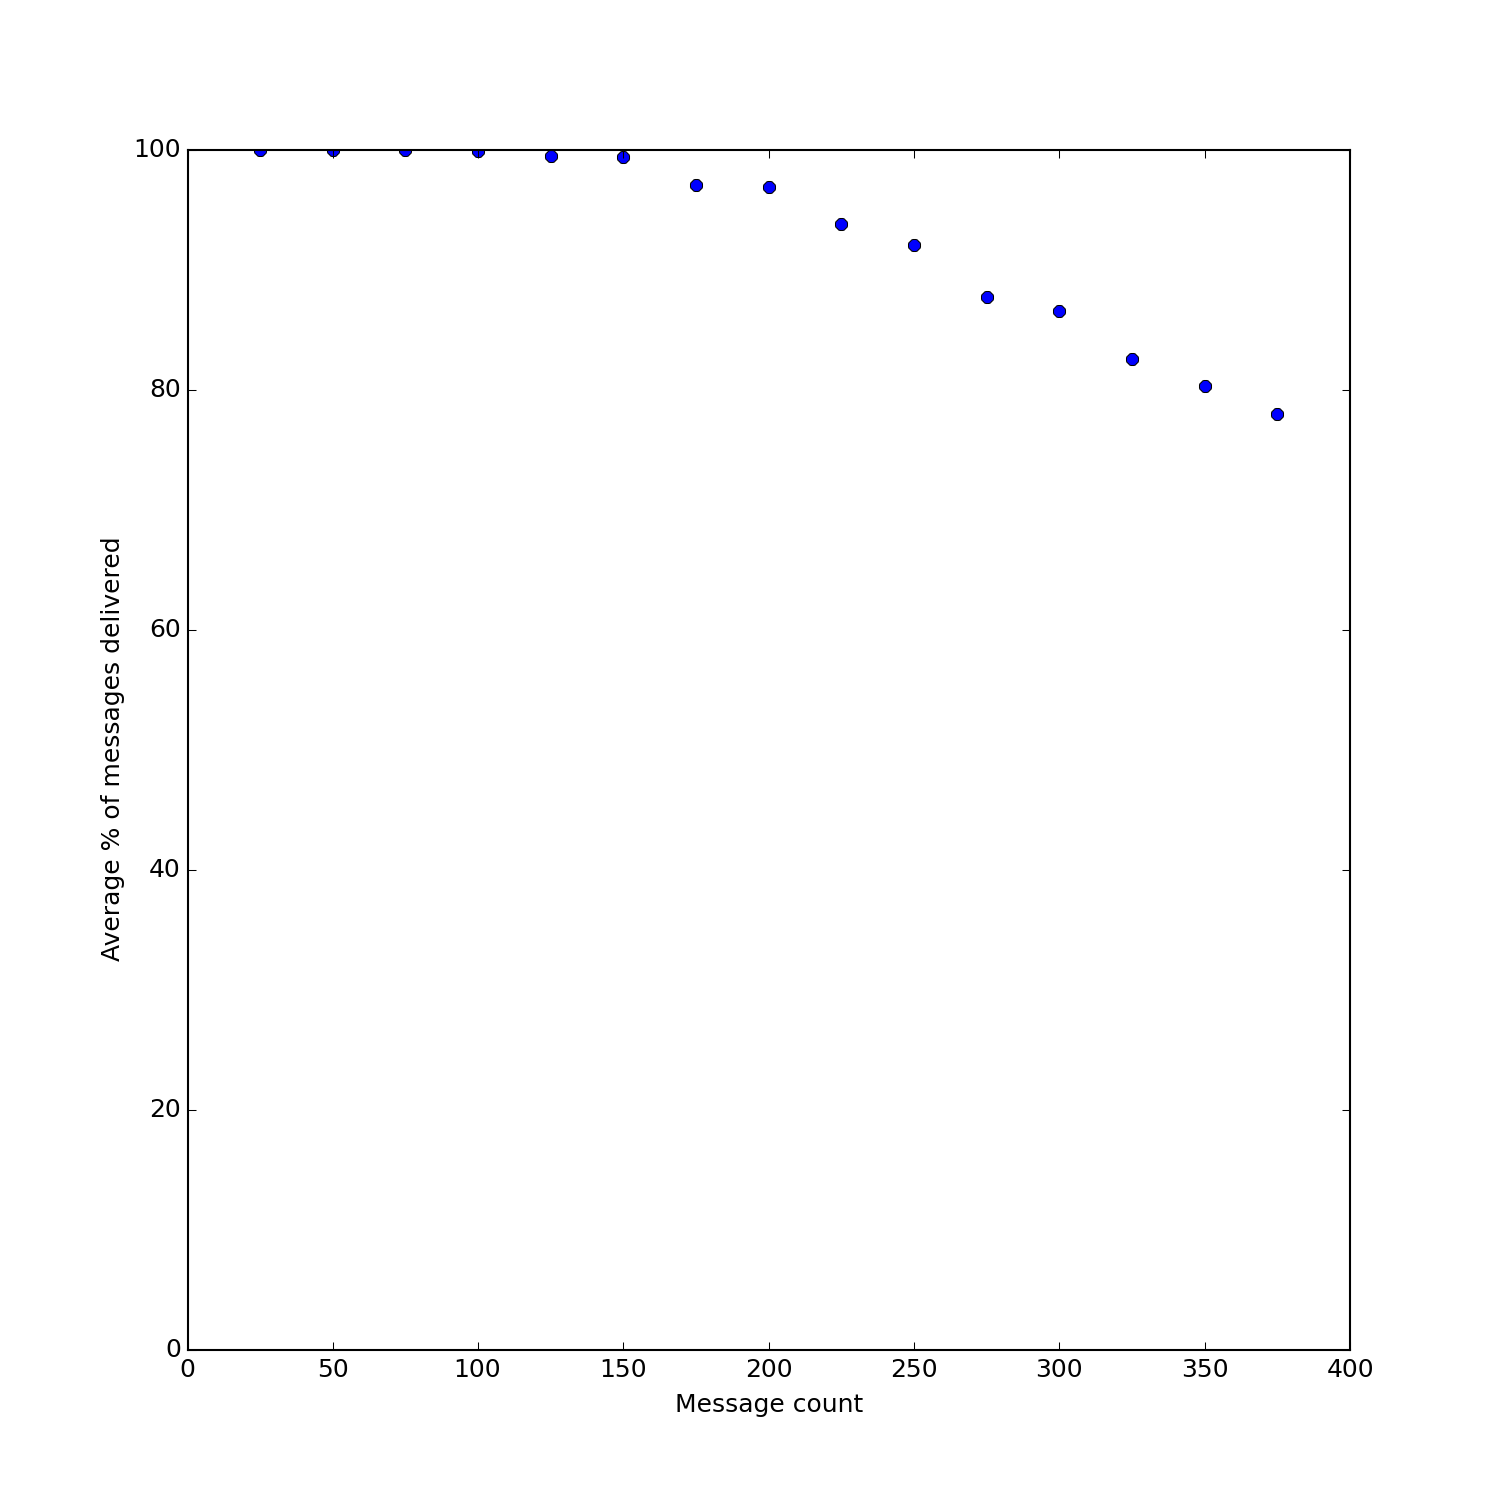
\includegraphics[width=\textwidth]{results/BasicShare_Prob40}
        \caption{Algorithm 2 (0.4)}
        \label{fig:results/BasicShare_Prob40}
    \end{subfigure}
    ~ %add desired spacing between images, e. g. ~, \quad, \qquad, \hfill etc. 
    %(or a blank line to force the subfigure onto a new line)
    

    \begin{subfigure}[b]{0.3\textwidth}
        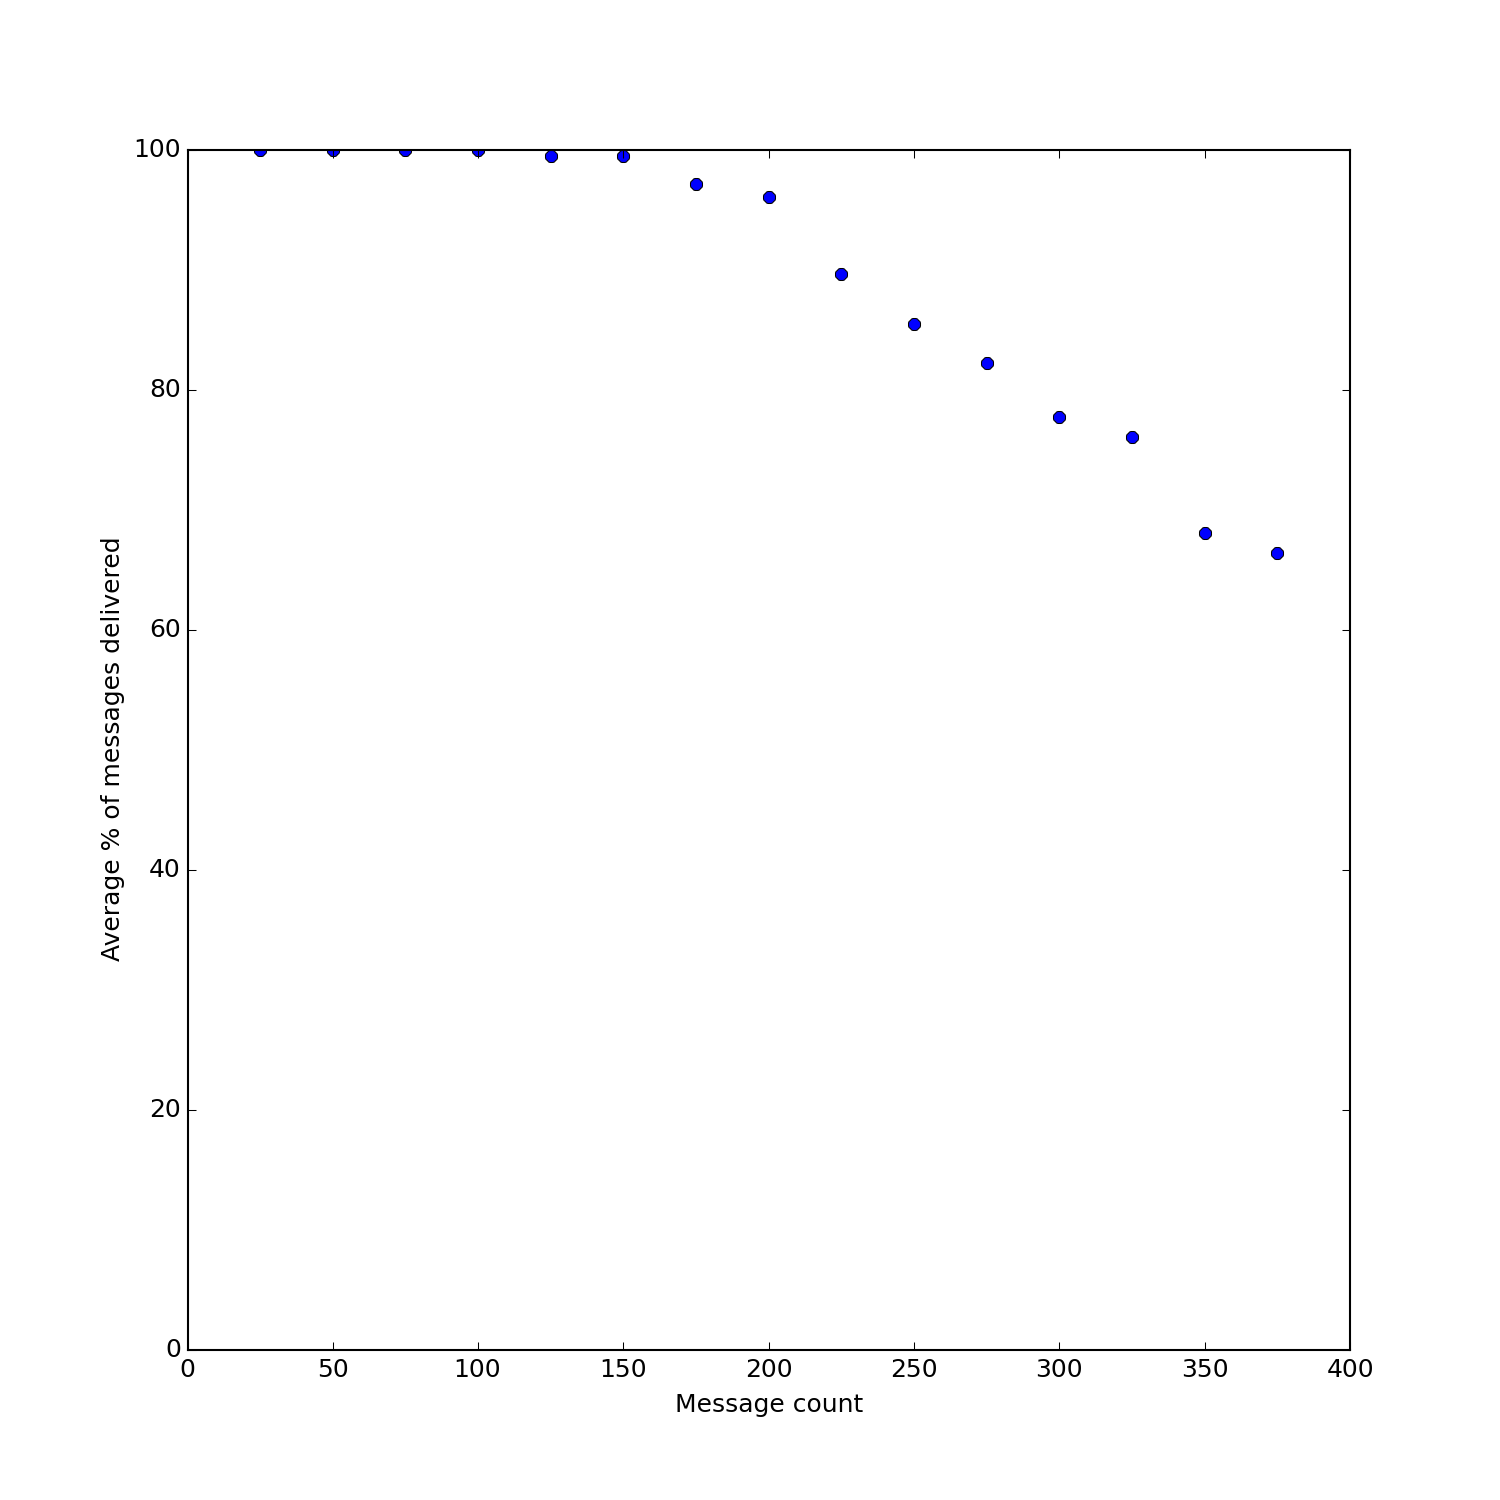
\includegraphics[width=\textwidth]{results/BasicShare_Prob60}
        \caption{Algorithm 2 (0.6)}
        \label{fig:results/BasicShare_Prob60}
    \end{subfigure}
    ~ %add desired spacing between images, e. g. ~, \quad, \qquad, \hfill etc. 
    %(or a blank line to force the subfigure onto a new line)
    \begin{subfigure}[b]{0.3\textwidth}
        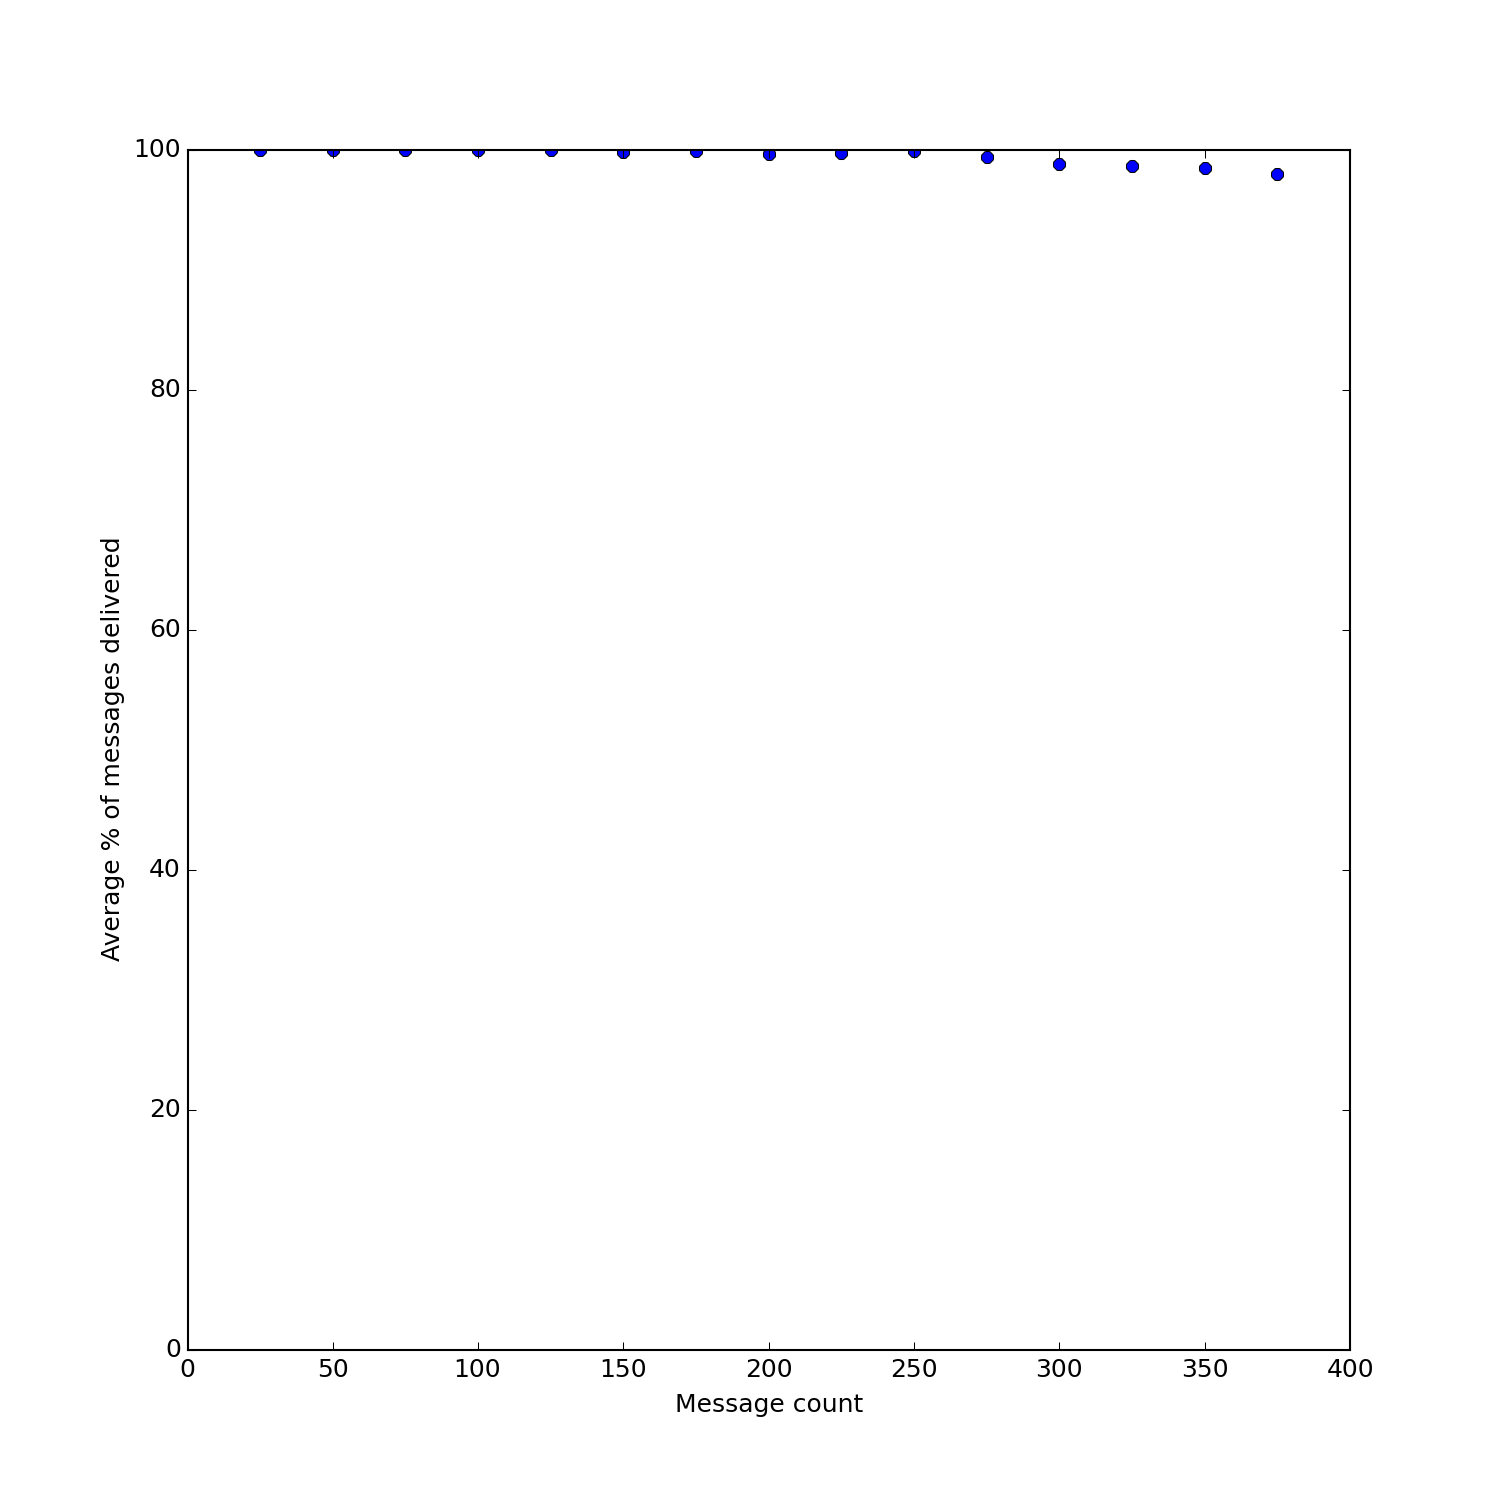
\includegraphics[width=\textwidth]{results/BasicShare_OnlyBest}
        \caption{Algorithm 3}
        \label{fig:results/BasicShare_OnlyBest}
    \end{subfigure}
  	\vspace{-5pt}
    \caption{Basic User Model}\label{fig:BasicUserModel}
  	\vspace{-15pt}
\end{wrapfigure}

\section{User Model Comparisons}
First the two user models were compared. In Figure 3.1 the results using the basic user model are shown. For these tests the user model parameters were $a = 20$ (maximum seen) and $b = 5$ (maximum shared). The number of messages was increased from 25 to 375 in increments of 25, and each simulation was repeated 10 times and the average taken. The graphs show this user model with various showing algorithms. These are: a) Algorithm 1 - Any closer node; b) Algorithm 2 - Further nodes with probability 0.4; c) Algorithm 2 - Further nodes with probability 0.6; d) Algorithm 3 - Only single best node. We can see that as the probability of spreading messages away from the target increases, the percent of messages delivered decreases. This can be interpreted as the extra messages only clogging up the system. Of particular note is Figure 3.1d, where only sending each message a single node achieves extremely high performance with almost no decrease as message count increases.

\begin{wrapfigure}{L}{0.65\textwidth}
  	\vspace{-15pt}
    \centering
    \begin{subfigure}[b]{0.3\textwidth}
        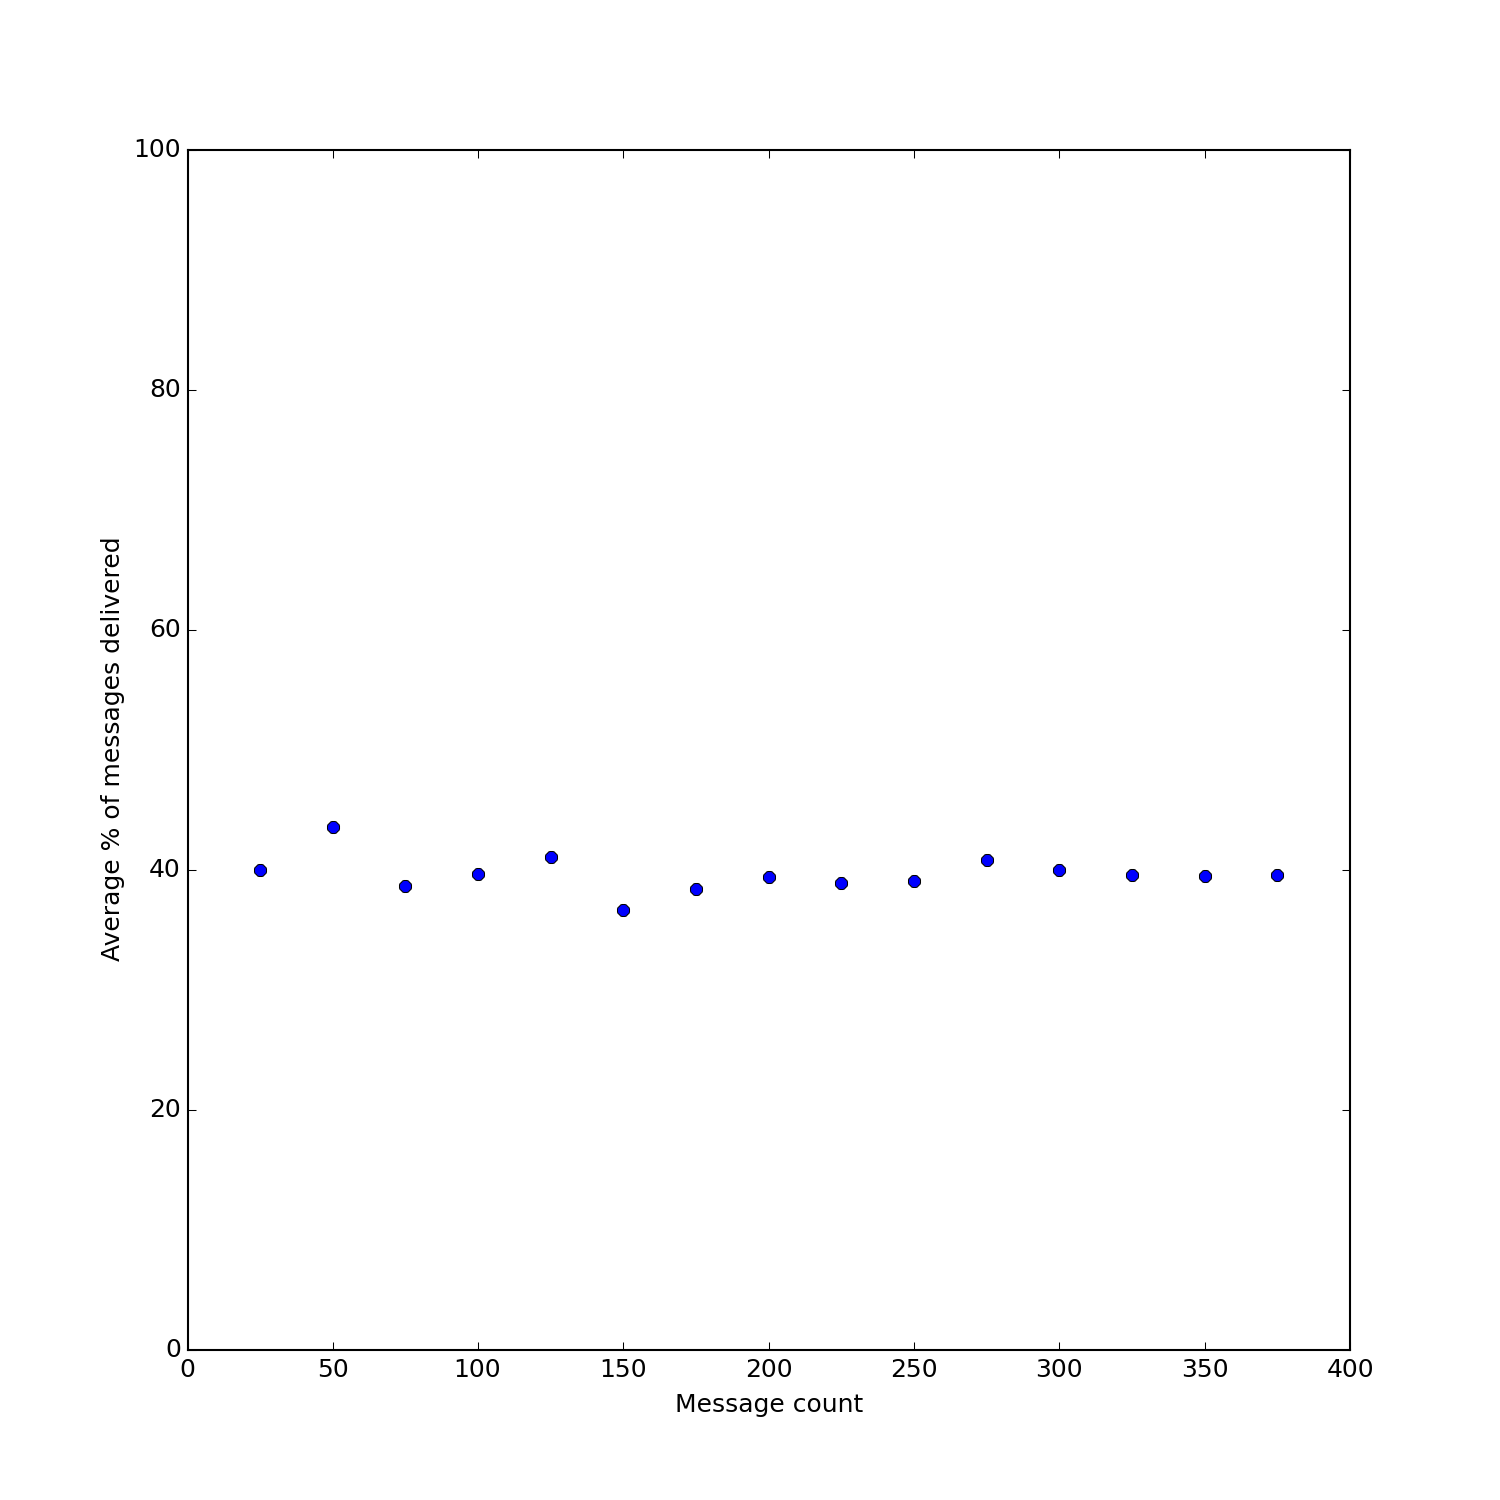
\includegraphics[width=\textwidth]{results/Prob50Share_Prob0}
        \caption{Algorithm 1}
        \label{fig:results/Prob50Share_Prob0}
    \end{subfigure}
    ~ %add desired spacing between images, e. g. ~, \quad, \qquad, \hfill etc. 
      %(or a blank line to force the subfigure onto a new line)
    \begin{subfigure}[b]{0.3\textwidth}
        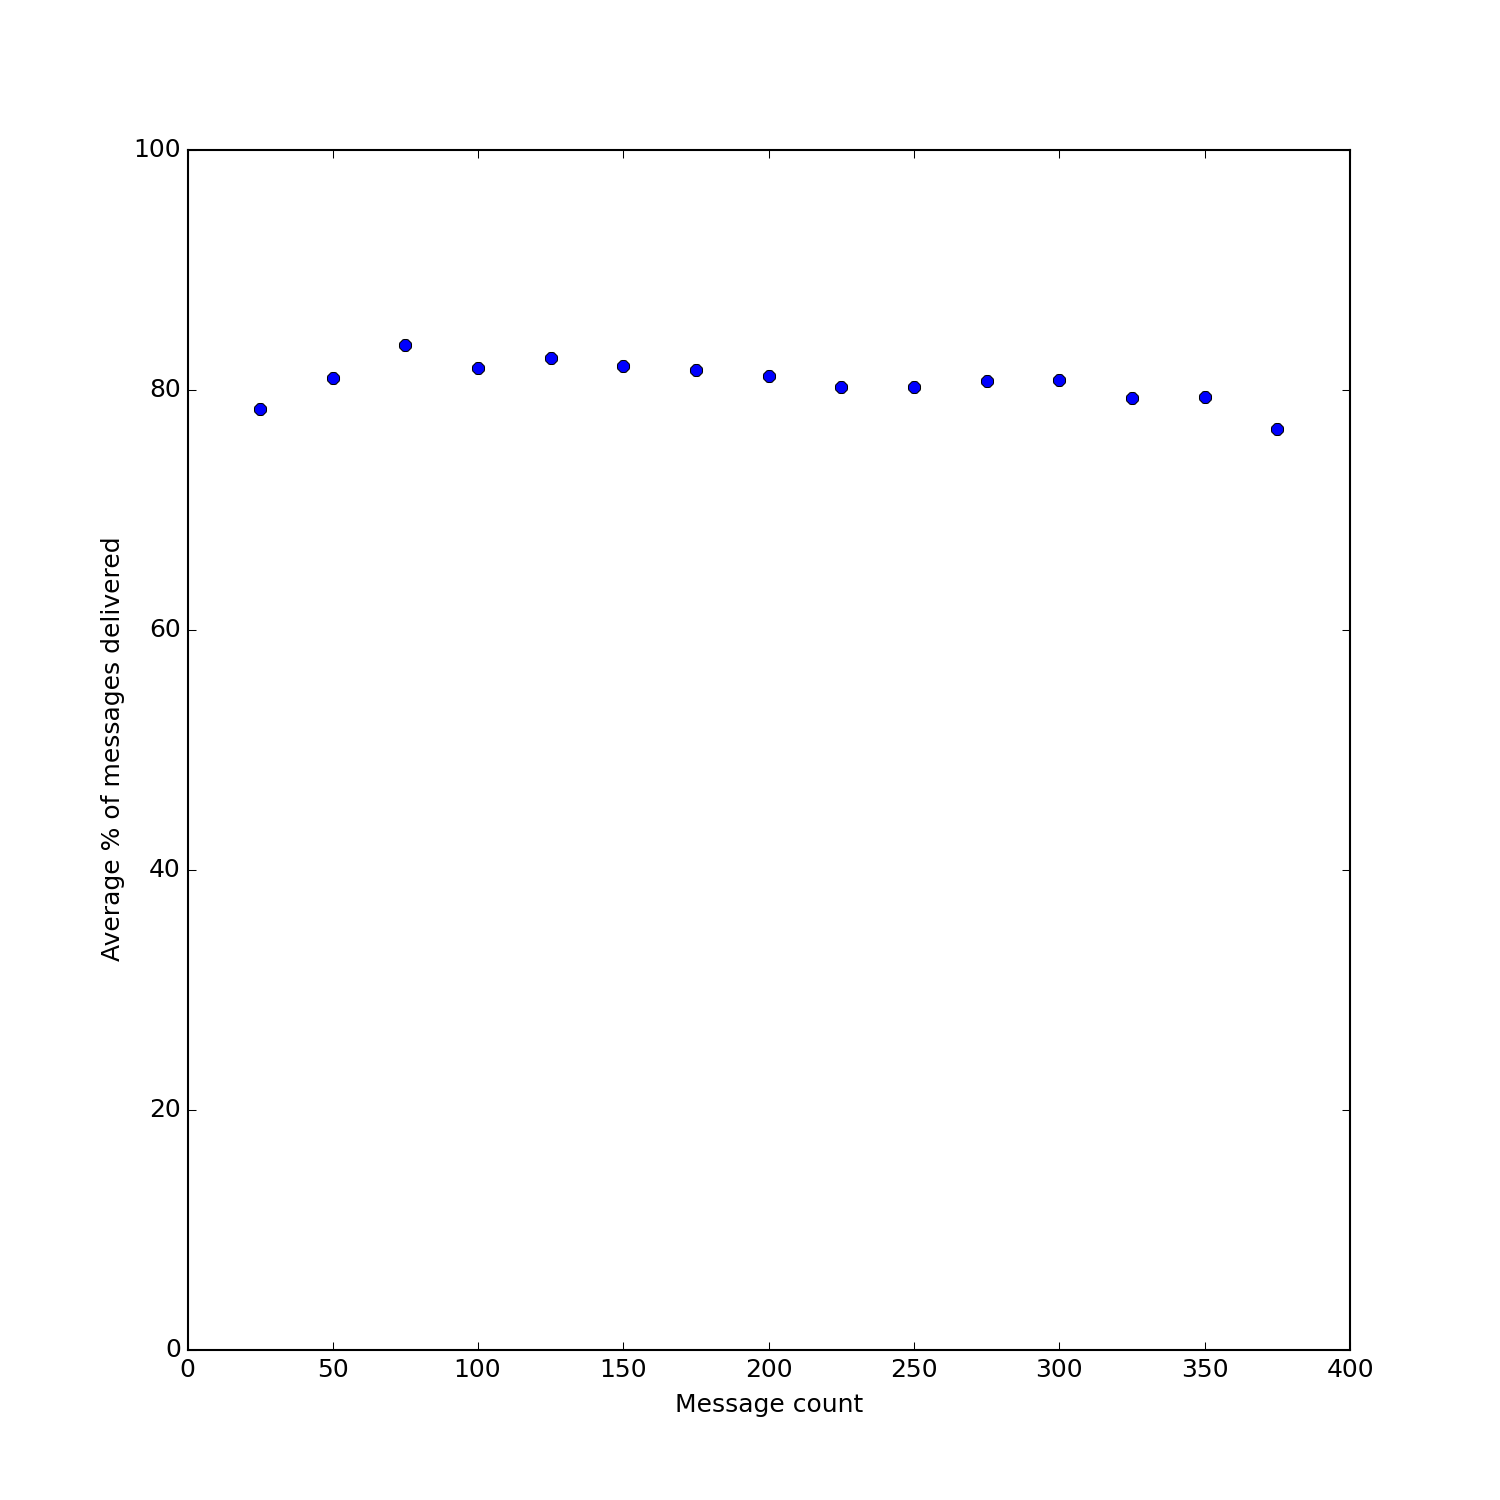
\includegraphics[width=\textwidth]{results/Prob50Share_Prob40}
        \caption{Algorithm 2 (0.4)}
        \label{fig:results/Prob50Share_Prob40}
    \end{subfigure}
    ~ %add desired spacing between images, e. g. ~, \quad, \qquad, \hfill etc. 
    %(or a blank line to force the subfigure onto a new line)
    
    
    \begin{subfigure}[b]{0.3\textwidth}
        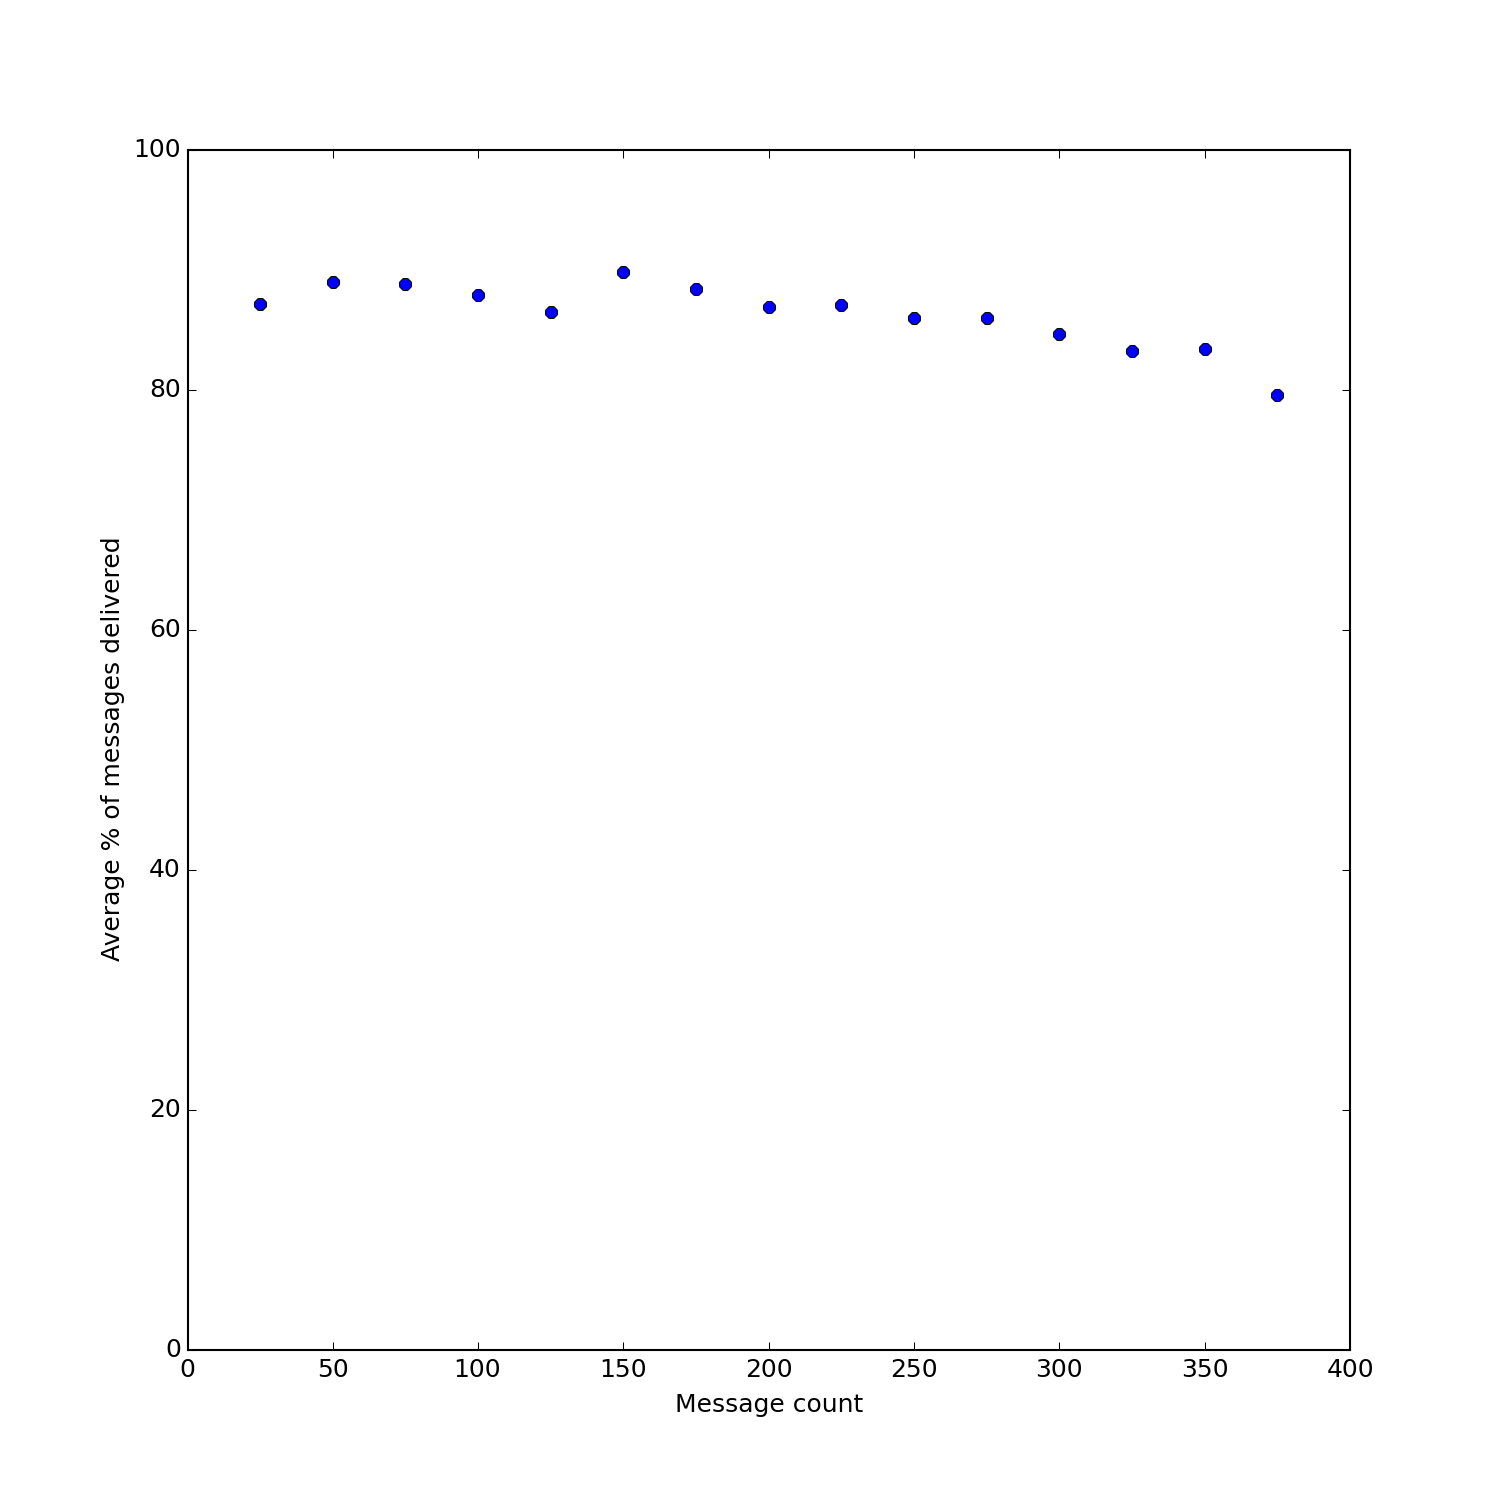
\includegraphics[width=\textwidth]{results/Prob50Share_Prob60}
        \caption{Algorithm 2 (0.6)}
        \label{fig:results/Prob50Share_Prob60}
    \end{subfigure}
    ~ %add desired spacing between images, e. g. ~, \quad, \qquad, \hfill etc. 
    %(or a blank line to force the subfigure onto a new line)
    \begin{subfigure}[b]{0.3\textwidth}
        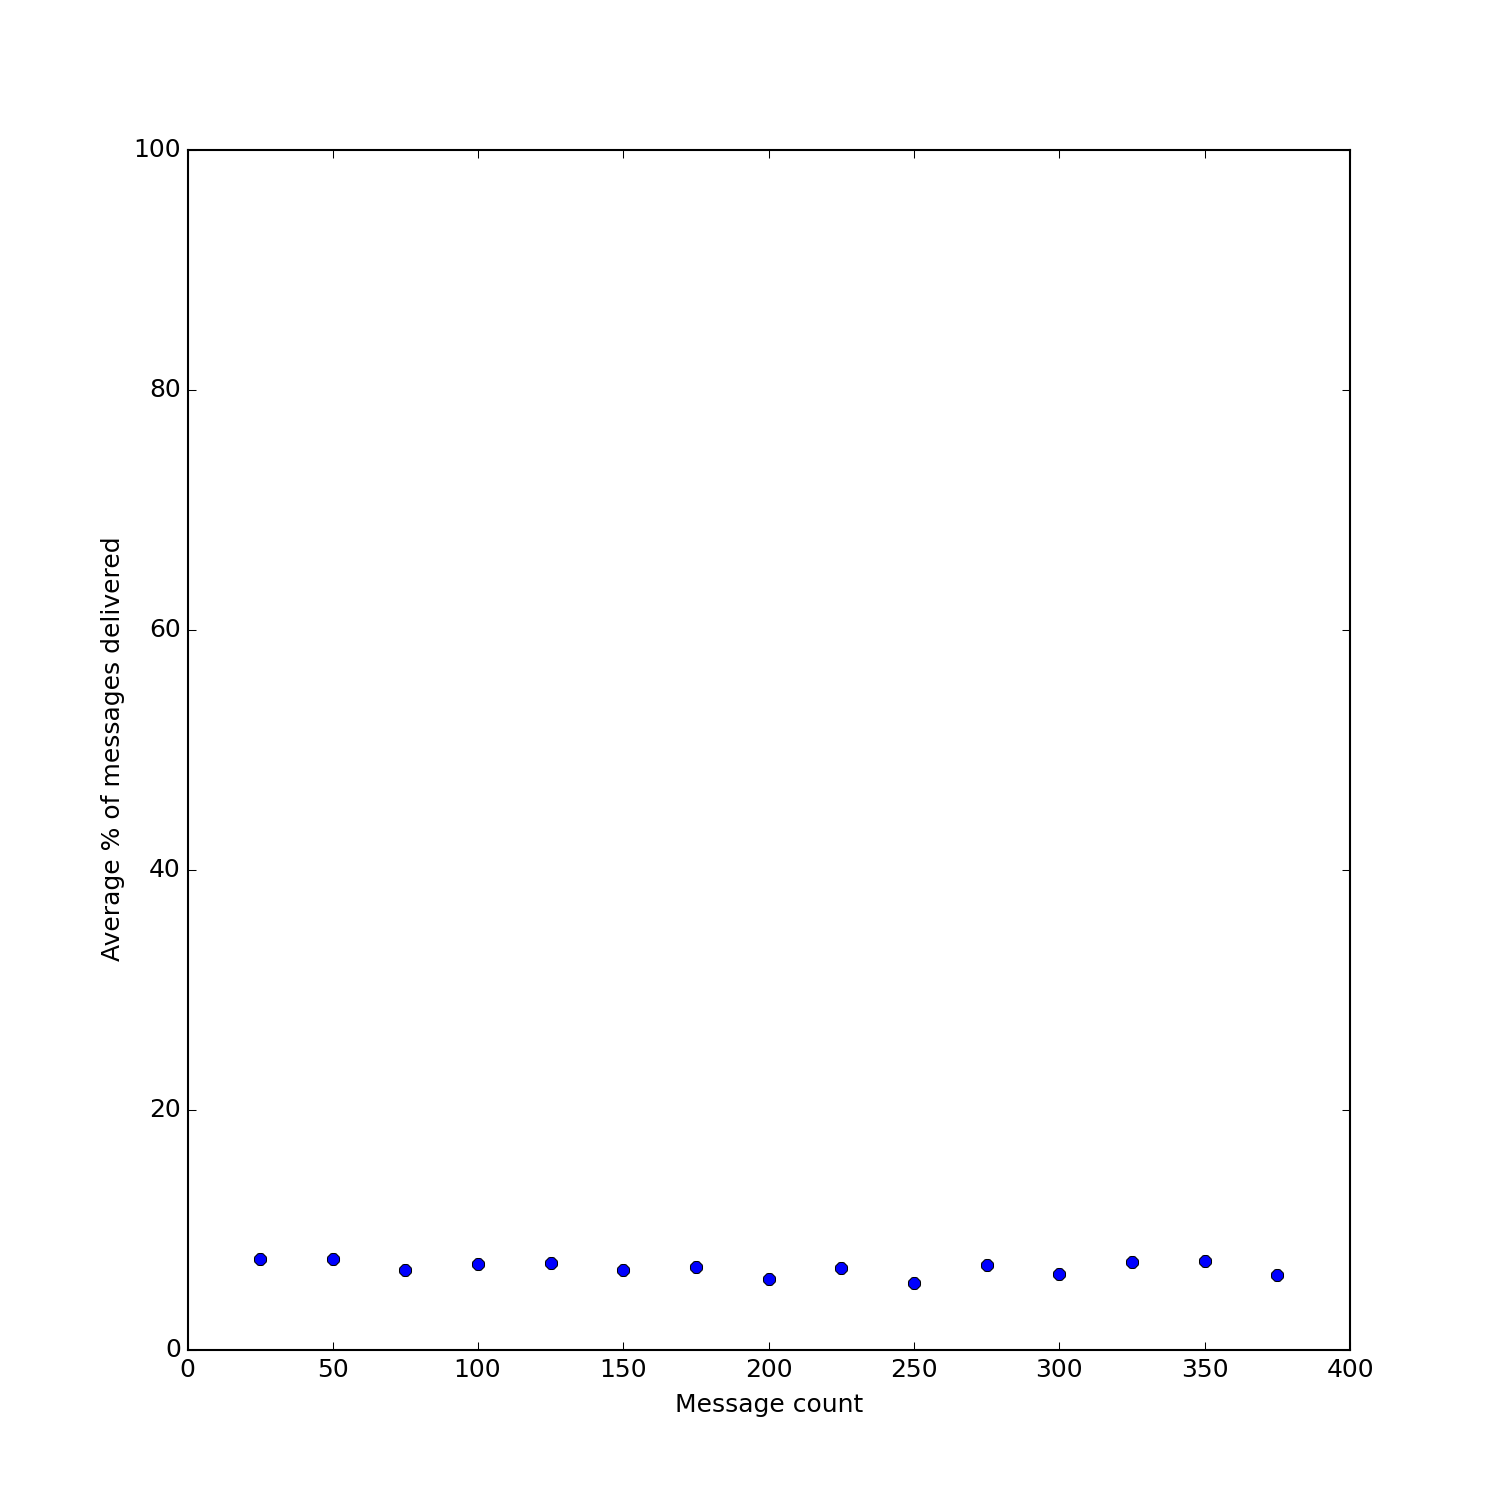
\includegraphics[width=\textwidth]{results/Prob50Share_OnlyBest}
        \caption{Algorithm 3}
        \label{fig:results/Prob50Share_OnlyBest}
    \end{subfigure}
  	\vspace{-5pt}
    \caption{Probabilistic User Model}\label{fig:Prob50UserModel}
  	\vspace{-15pt}
\end{wrapfigure}

Contrasting this in Figure 3.2 are results using the probabilistic user model, with $a = 20$ (maximum seen) and $p = 0.5$ (probability of sharing). The same message counts and repetitions were used. Graphs a--d show this user model with the same respective showing algorithms as Figure 3.1. In this case we see almost the opposite - as the probability of sharing the message away from the target increases, so does the percentage of messages delivered. Figure 3.2d shows that Algorithm 3 does particularly badly in this case, delivering almost no messages. In general the message count has less of an effect than before, suggesting that messages not being passed on is now more of a problem than congestion.

These results taken together, particularly looking at Algorithm 3, suggest that the basic user model is not as accurate a model when the message count is low - even if users are shown few messages, they would be unlikely to share all of them. In the rest of the experiments, the probabilistic user model is used for this reason.


\section{Algorithm 2 Further Node Probability}
The next tests run looked at how changing the probability of sending a message in a direction not closer to the target affects the delivery rate. These tests were again repeated 10 times each, and used the probabilistic user model with $a = 20$ and $p = 0.5$. Three sets of simulations were run, with message counts of 200, 400 and 800. In each of these, the probability parameter for showing algorithm 2 was increased from 0.1 to 1.0 in 0.1 increments. The results can be seen in Figure 3.3.

\begin{figure}[h]
  	\vspace{-10pt}
    \centering
    \begin{subfigure}[b]{0.3\textwidth}
        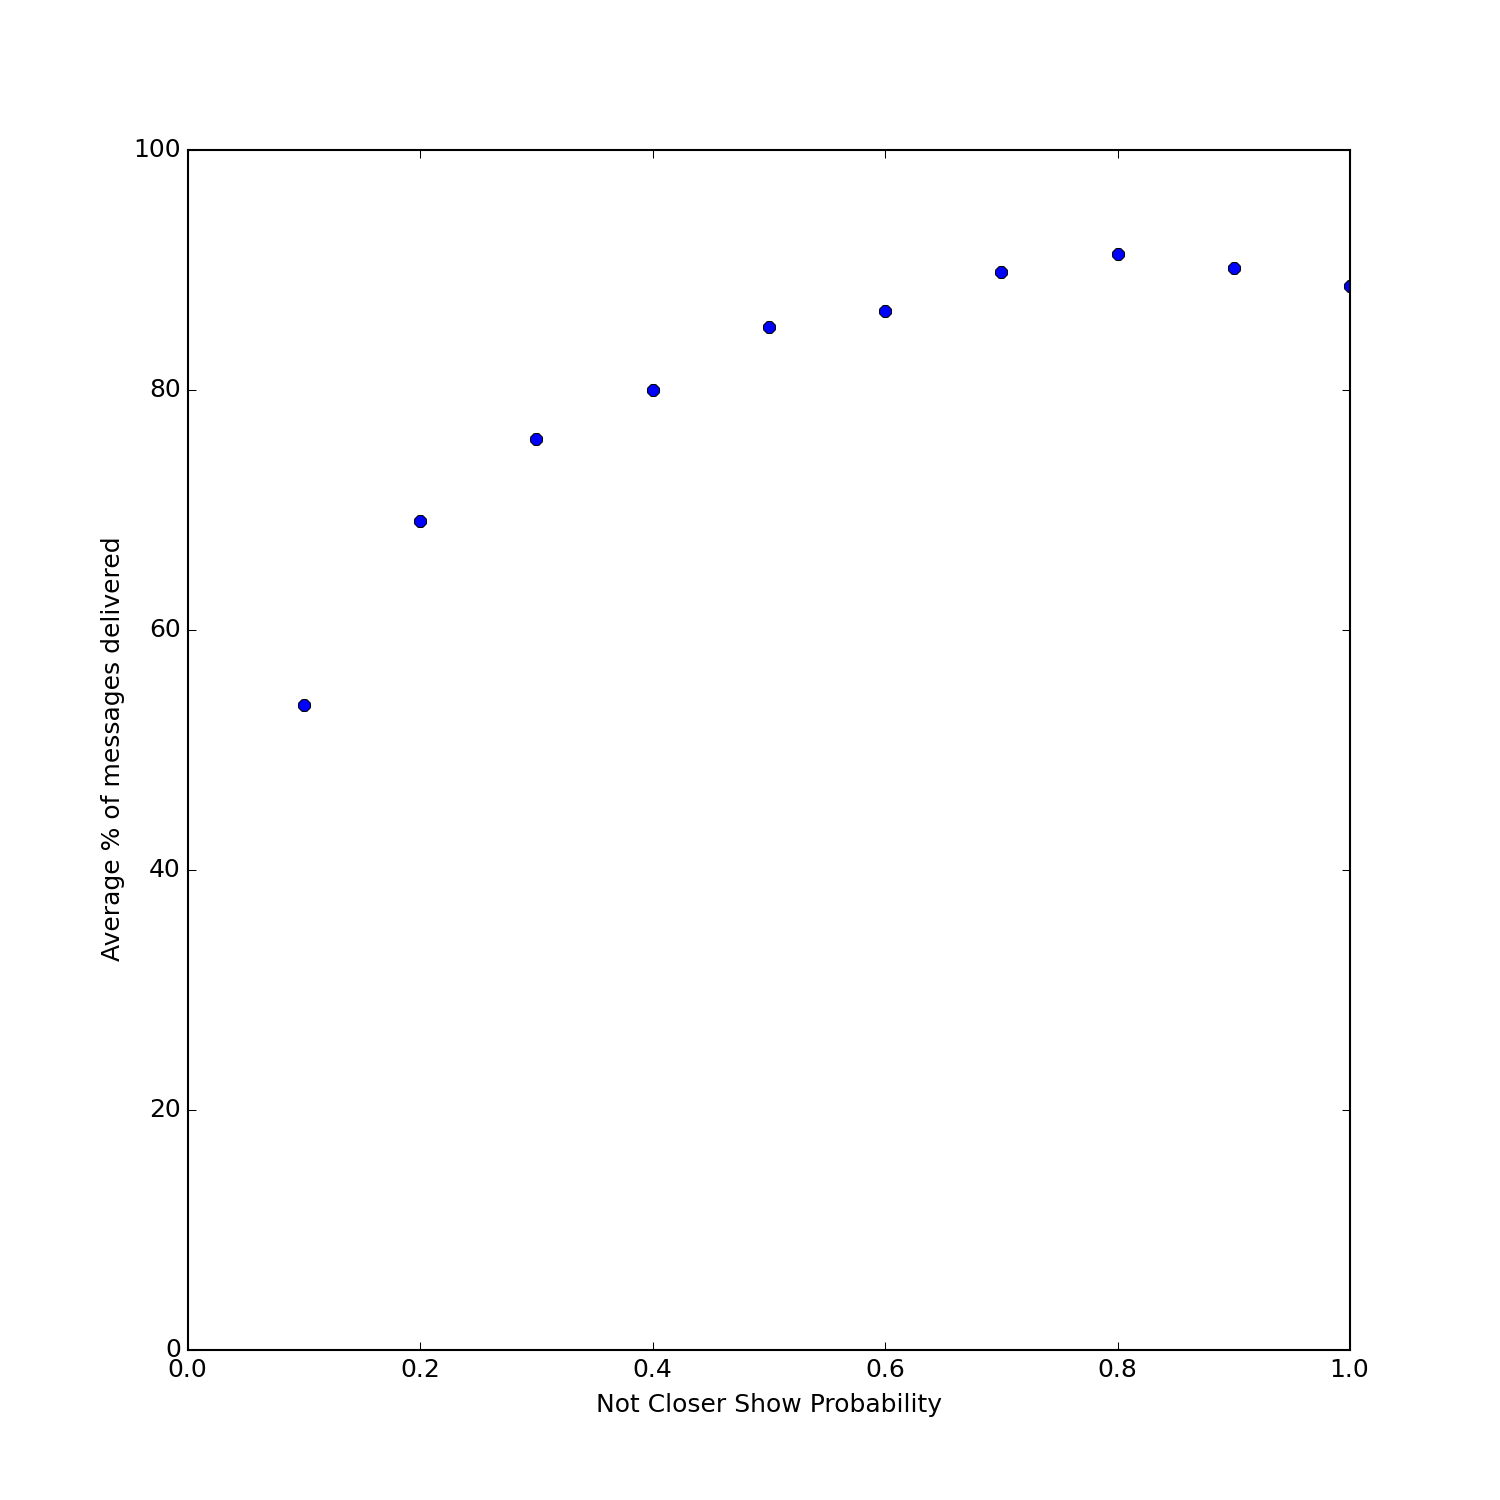
\includegraphics[width=\textwidth]{results/notCloserProb_200messages}
        \caption{200 Messages}
        \label{fig:results/notCloserProb_200messages}
    \end{subfigure}
    ~ %add desired spacing between images, e. g. ~, \quad, \qquad, \hfill etc. 
      %(or a blank line to force the subfigure onto a new line)
    \begin{subfigure}[b]{0.3\textwidth}
        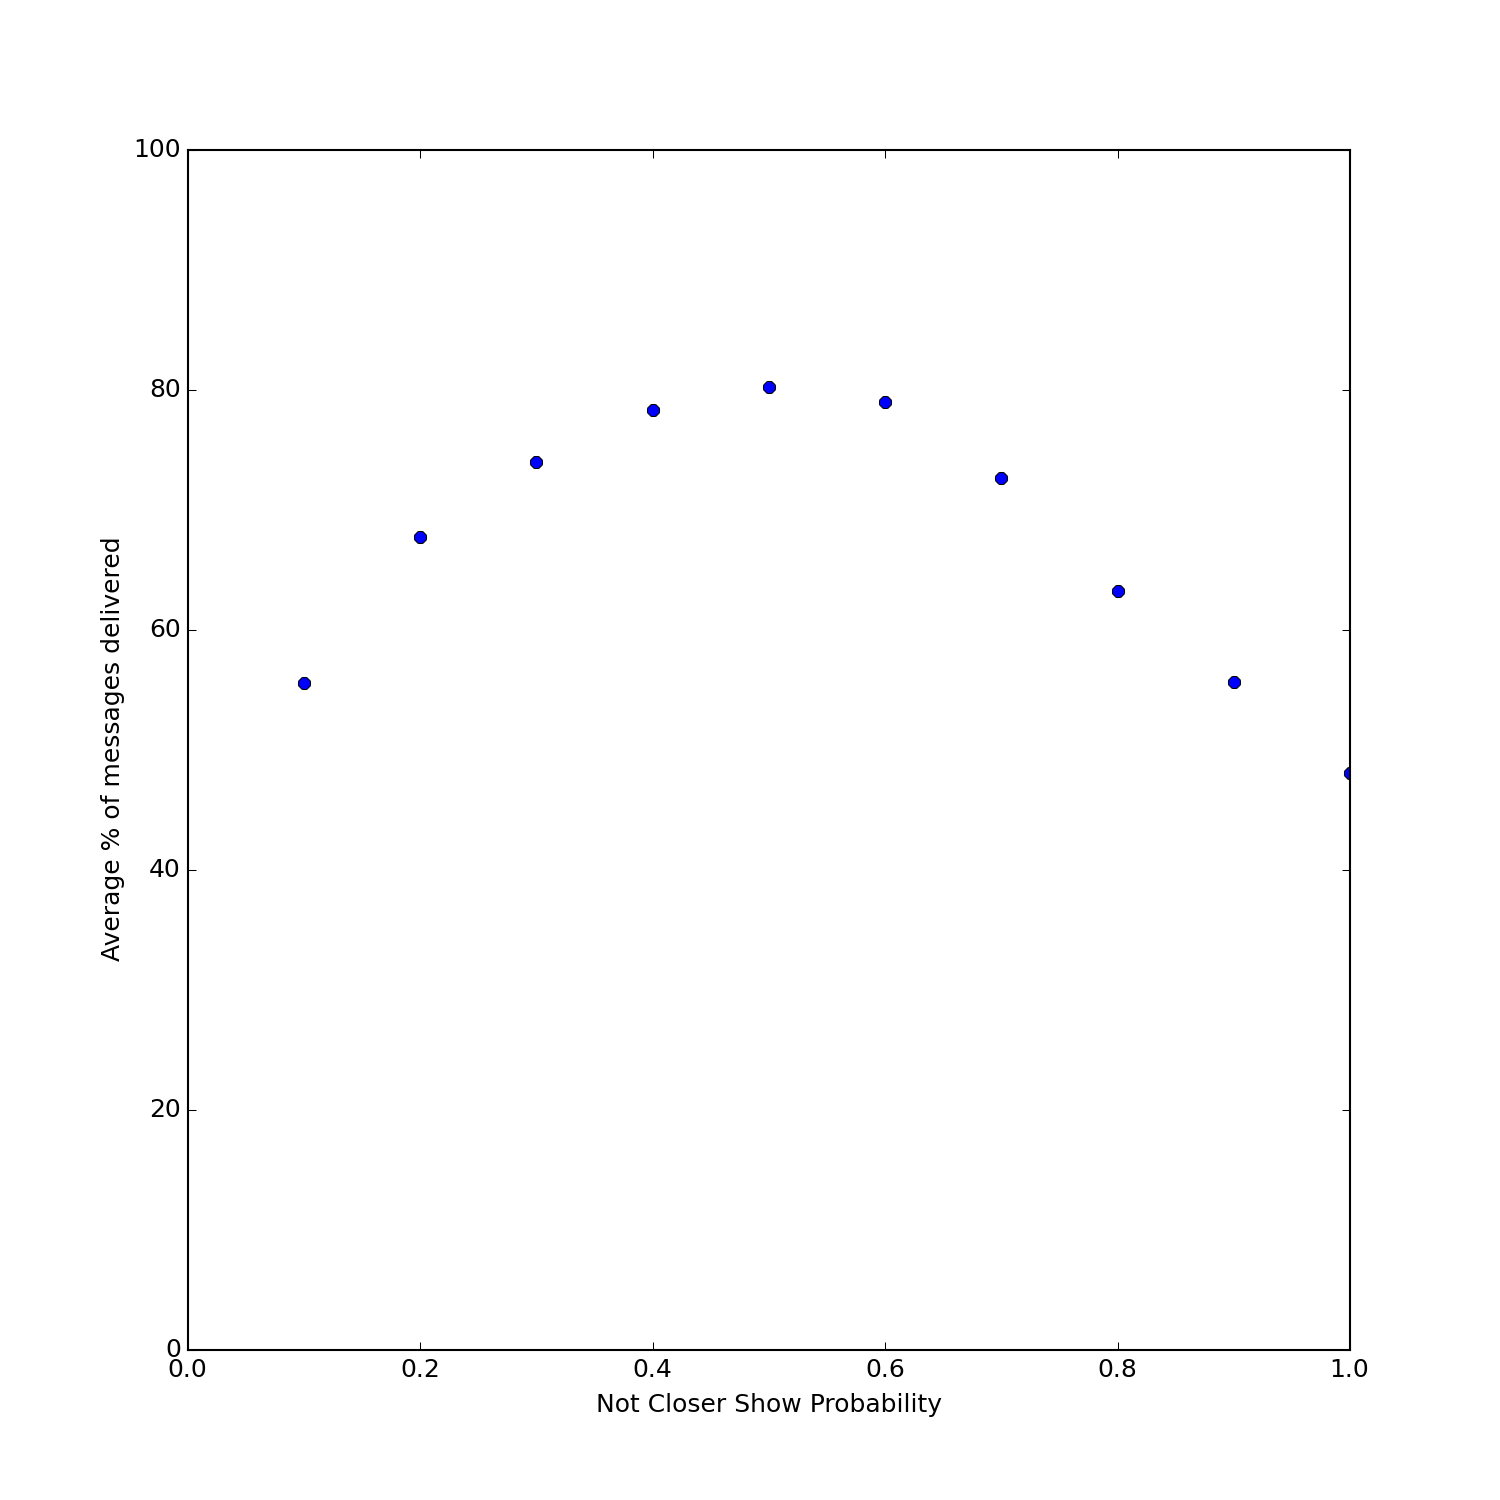
\includegraphics[width=\textwidth]{results/notCloserProb_400messages}
        \caption{400 Messages}
        \label{fig:results/notCloserProb_400messages}
    \end{subfigure}
    ~ %add desired spacing between images, e. g. ~, \quad, \qquad, \hfill etc. 
    %(or a blank line to force the subfigure onto a new line)
    \begin{subfigure}[b]{0.3\textwidth}
        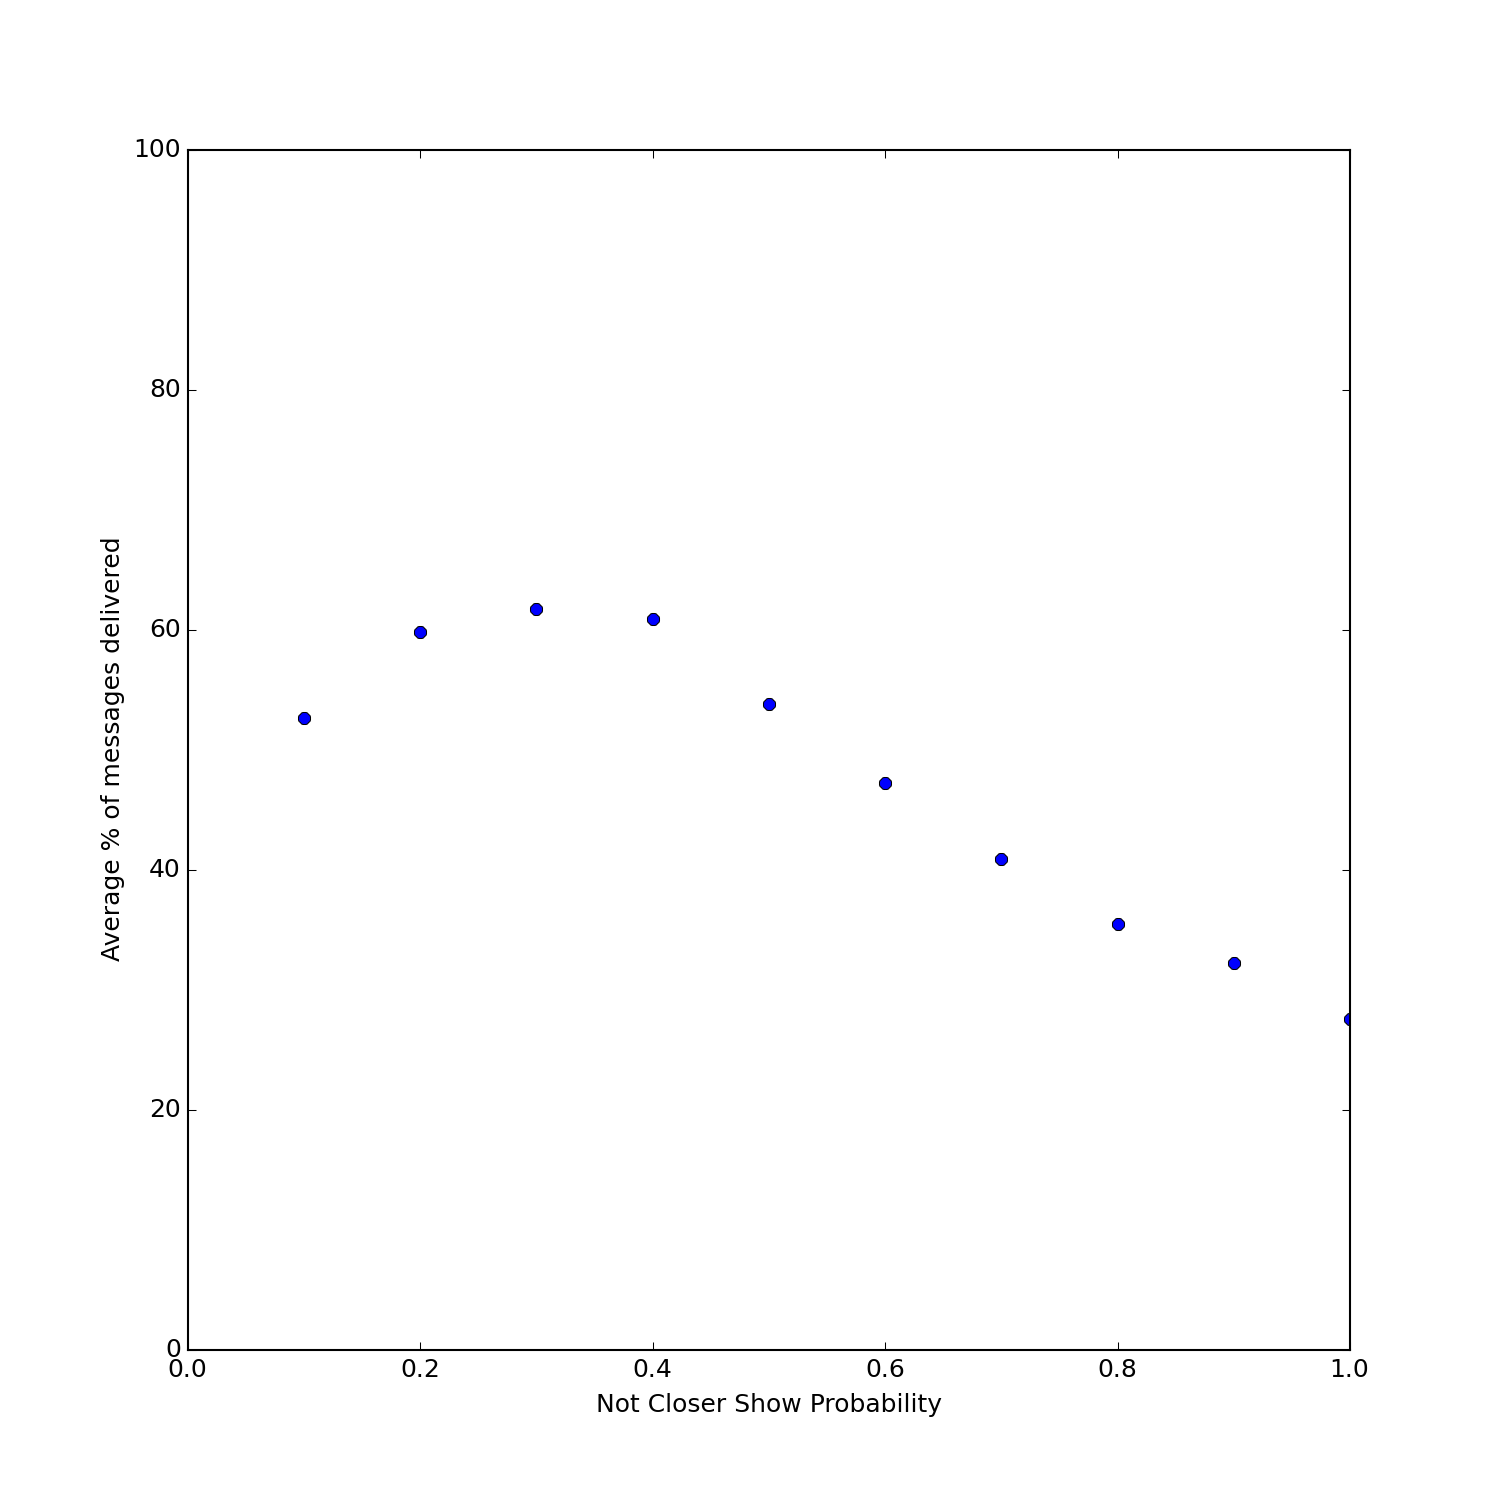
\includegraphics[width=\textwidth]{results/notCloserProb_800messages}
        \caption{800 Messages}
        \label{fig:results/notCloserProb_800messages}
    \end{subfigure}
  	\vspace{-5pt}
    \caption{Not Closer Probability}\label{fig:NotCloserProbability}
  	\vspace{-5pt}
\end{figure}

In these results it can be seen that, unsurprisingly, those with a higher number of messages had a generally lower delivery rate. More interesting is the point at which the delivery rates "peak" as the showing probability increases. All 3 cases show this peak, with it being at around 0.8 for 200 messages, 0.5 for 400 messages, and 0.3 for 800 messages. Also interesting is the fact that the delivery rates in all 3 graphs follow a similar trend up to their peak. This suggests that depending on how many messages there are, spreading messages further increases the chance of delivery up to a point where there a simply too many messages in the system. Once this point is reached, the delivery rates fall faster if the messages are spread more. This is an observation that should prove useful when considering other algorithms in the future.


\chapter{Future Plan}
\section{Further Work}

\subsection{Further Algorithms}
One of the main things to be expanded is the development of other message showing algorithms. By using slightly more sophisticated methods it may be possible to achieve improved performance compared to the basic methods tested so far. For example, the current algorithms differentiate between whether or not messages get closer to the destination, but not how much they get closer by. Since the long jumps play an important role in getting the message to the destination, it may be advantageous to prioritise these. Additionally 

\subsection{Other Graph Types}
Up to this point, algorithms have only been tested on Kleinberg's small world graph model. However it may provide useful results to test them on other graphs. 

Simple graphs such trees or a grid may provide a baseline to compare the results received so far against, and may also provide useful opportunities to perform analysis on the process. Alternatively, other models that are used to describe social networks such as preferential attachment may provide an alternative perspective for testing the algorithms. Finally it would be interesting to use an actual social network, such as those in the SNAP library\cite{snapnets}, may show if the algorithms have potential in real-world settings, rather than being too heavily crafted for the model used in simulations.

\subsection{Analysis}
Beyond simply developing and testing various algorithms, it will be useful to perform analysis on the problem to conclude something more definite. Firstly, it may be possible to find an upper bound on how many messages it is possible to deliver in the best case. By working on this upper bound to lower it as much as possible, this will provide an idea of the optimal possible performance, which the algorithms developed can then be compared to.

Additionally, it will useful to compare the performance of this message delivering system to network flow on the same graph. Although there are some differences, if there is a constant flow of messages coming into the system then this is somewhat similar to the idea of a multi-commodity network flow where there are multiple flows between source and sink nodes. The algorithms can be first compared to network flow experimentally, by measuring their performances. After this, if time allows, it may be possible to perform additional theoretical analysis comparing the two - by comparing the performance bounds of each.


\section{Plan for Semester 2}
ToDo
\chapter{Conclusion}
ToDo

% use the following and \cite{} as above if you use BibTeX
% otherwise generate bibtem entries
\bibliographystyle{plain}
\bibliography{interimBib}


\end{document}
